\documentclass[conference]{IEEEtran}
\usepackage[T1]{fontenc}
\usepackage[utf8]{inputenc}
\usepackage{amsmath,amssymb}
\usepackage{graphicx}
\usepackage{booktabs}
\usepackage{multirow}
\usepackage{cite}
\usepackage[hidelinks]{hyperref}

% Compact tables so that they stay inside one IEEE column.
\newcommand{\tabstyle}{\footnotesize\setlength{\tabcolsep}{3.5pt}}

\begin{document}

\title{Emotion-Aware Speech Recognition with Separate ASR and Emotion Models}

\author{\IEEEauthorblockN{Hoang Thien Nhan}
\IEEEauthorblockA{25C11054\\
25C1105417@student.hcmus.edu.vn}
\and
\IEEEauthorblockN{Lam Thinh Phat}
\IEEEauthorblockA{25C11058\\
25C1105836@student.hcmus.edu.vn}}

\maketitle

\begin{abstract}
Emotion-aware speech recognition has to output what a speaker says and how the speaker feels. When one model is
trained for both tasks, the two objectives compete. When emotion is recognized from automatic transcripts, every
recognition error is passed on to the emotion classifier. We keep the two tasks in separate models. A finetuned
Whisper model transcribes the speech. A second model predicts the emotion from that transcript, the previous
turns of the dialogue and the audio, which a frozen speech encoder turns into features. A gated fusion combines
the text and audio features. We choose each component with a controlled comparison and then remove each part of the
emotion model to measure what it adds. On IEMOCAP with leave-one-session-out evaluation, finetuning changes which
recognizer is best, and the Whisper encoder works better than WavLM as the audio branch. Text, dialogue context and
audio each improve emotion recognition, and text helps the most. One Whisper model serves as both the recognizer and
the audio encoder. Replacing automatic transcripts with ground-truth text improves emotion recognition only slightly,
with or without the audio branch, and much less than adding audio or dialogue context does. At the error rate of a
finetuned recognizer, audio and context are therefore worth more than a further reduction in word error rate.
\end{abstract}

\begin{IEEEkeywords}
speech emotion recognition, automatic speech recognition, Whisper, multimodal fusion, IEMOCAP
\end{IEEEkeywords}

\section{Introduction}

Emotion-aware speech recognition takes one utterance and returns two outputs, the words (automatic speech
recognition, ASR) and the speaker's emotion (speech emotion recognition, SER). Existing systems follow one of two
designs. The first trains a single model for both tasks, for example a speech encoder with an ASR head and an emotion
head \cite{cai2021mtl,shen2024ent,chen2025vibemo}. The second runs ASR first and recognizes emotion from the
transcript, usually together with the audio \cite{li2024asrtranscripts,he2024mfaedaec}.

Each design has a weakness. In joint training, the two tasks pull the shared network in different directions, and
the network tends to favor ASR \cite{gao2023twostage}. In the pipeline, ASR errors reach the emotion classifier, and
the damage grows with the word error rate (WER) \cite{li2024asrtranscripts}.

We build a system from two separate models and measure each design choice. The audio goes to two branches in
parallel. The text branch transcribes the audio with an ASR model and reads the transcript together with the previous
dialogue turns. The audio branch encodes the same audio with a frozen speech encoder. A gated fusion combines the two
branches and a classifier predicts the emotion. Our contributions are:
\begin{itemize}
  \item a controlled comparison of two ASR models, before and after finetuning, on the same folds;
  \item an SER system that reads ASR transcripts, dialogue context and audio;
  \item an ablation of every part of the emotion model, and a measurement of what ASR errors cost.
\end{itemize}

\section{Background}

\textbf{Joint models.} Cai et al.\ \cite{cai2021mtl} add a CTC head for ASR next to the emotion classifier on
wav2vec 2.0. The Emotion Neural Transducer \cite{shen2024ent} extends an RNN-T with an emotion joint network.
VIB-Emo \cite{chen2025vibemo} finetunes an LLM to predict emotion, speech descriptors and the transcript together.
Gao et al.\ \cite{gao2023twostage} report that multi-task training suffers from gradient conflict. They learn ASR in
a first stage and emotion in a second.

\textbf{SER from ASR transcripts.} Li et al.\ \cite{li2024asrtranscripts} benchmark eleven ASR systems and several
fusion methods on IEMOCAP and two other corpora. Transcripts with about 10\% WER give results close to ground-truth
text. MF-AED-AEC \cite{he2024mfaedaec} adds ASR error detection and correction as auxiliary losses to an audio-text
model.

\textbf{Speech encoders and context.} In the EmoBox benchmark \cite{ma2024emobox}, the Whisper large-v3 encoder
reaches a higher UA on IEMOCAP than WavLM-large under the same probe (73.54 vs 69.47). Systems in the GenSEC
challenge show that previous dialogue turns improve text-only emotion recognition \cite{zhang2024contextual}.

Table~\ref{tab:related} lists published systems on IEMOCAP. Their data splits, validation sets and metrics differ, so
the numbers are not directly comparable.

\begin{table*}[!t]
\centering
\caption{Published systems on IEMOCAP (4 classes). ``Transcript'' means that the emotion model reads automatic
transcripts. Data splits and metrics differ between papers, so the numbers are not directly comparable.}
\label{tab:related}
\begin{tabular}{llccccc}
\toprule
System & Type & Transcript & Audio & Context & WER (\%) & UA (\%) \\
\midrule
Gao et al.\ 2023 \cite{gao2023twostage} & multi-task training & -- & \checkmark & -- & -- & 76.10 \\
ENT \cite{shen2024ent} & one model, ASR + SER & -- & \checkmark & -- & 26.47 & 73.88 \\
VIB-Emo \cite{chen2025vibemo} & one LLM, ASR + SER & -- & \checkmark & -- & 11.1 & 77.6 \\
MF-AED-AEC \cite{he2024mfaedaec} & ASR first, then SER & \checkmark & \checkmark & -- & 20.48 & 79.3 \\
EmoBox, Whisper large-v3 \cite{ma2024emobox} & audio only & -- & \checkmark & -- & -- & 73.54 \\
PL-Distill \cite{yang2026pldistill} & audio only, learned from an LLM & -- & \checkmark & -- & -- & 83.91 \\
Crab \cite{ueda2026crab} & ground-truth text + audio & -- & \checkmark & -- & -- & 75.85 \\
\midrule
Our system & ASR first, then SER & \checkmark & \checkmark & \checkmark & \textbf{9.56} & 81.17 \\
\bottomrule
\end{tabular}
\end{table*}

\textbf{Implications for our study.} Joint training suffers from gradient conflict \cite{gao2023twostage}, so we keep ASR
and SER in separate models and choose each one on its own metric. Whisper-style encoders beat WavLM in EmoBox, so we
compare both inside our system. Previous turns help text-based emotion recognition, so the text branch reads them.
We train on one GPU, so the audio encoder stays frozen.

\section{Method}

\subsection{Overview}

The system has two separate models. One is the ASR model. The other predicts emotion from three inputs, the ASR
transcript, the previous dialogue turns and the audio. Fig.~\ref{fig:overview} shows how they connect. The audio goes
into two branches in parallel. The text branch turns it into a transcript and encodes the transcript with its
dialogue context. The audio branch encodes the signal directly with a frozen encoder. A gated fusion combines the two
vectors, and a classifier predicts one of four emotions. The transcript is also the first output of the system.

\begin{figure*}[!t]
\centering
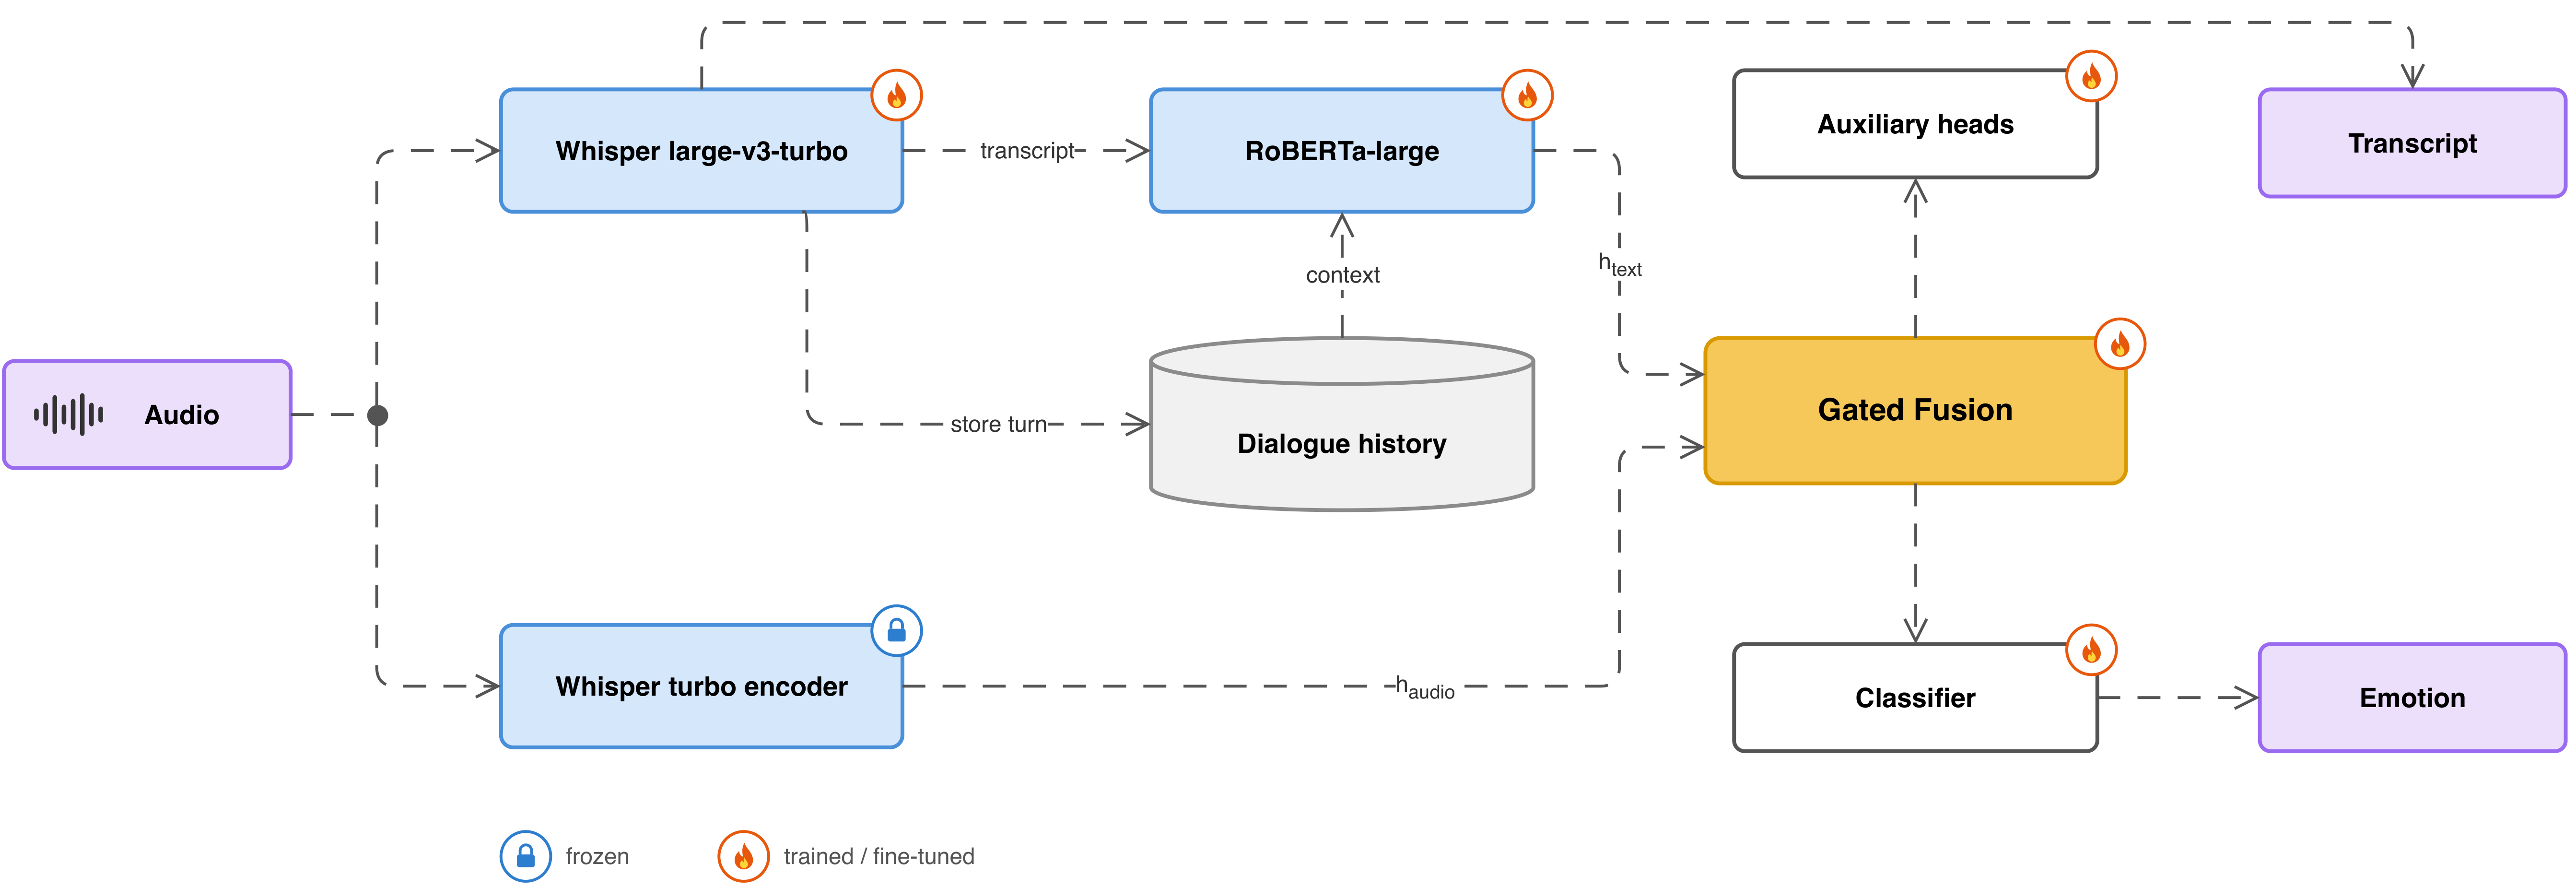
\includegraphics[width=0.85\textwidth]{figures/fig_overview.png}
\caption{System overview. The text branch consists of the ASR model, the dialogue history and RoBERTa-large. The
audio branch is the frozen Whisper encoder. A gated fusion combines the two branches. The auxiliary heads are used
only in training.}
\label{fig:overview}
\end{figure*}

\subsection{Text branch}

The text branch has three steps, shown on the left of Fig.~\ref{fig:flow}.

\textbf{Transcript.} We use Whisper large-v3-turbo \cite{radford2023whisper}, fully finetuned on the training sessions
of each fold. Turbo keeps the 32-layer encoder of Whisper large-v3 and cuts the decoder from 32 to 4 layers (809M
parameters in total) to speedup the decoding. In each fold, Whisper is finetuned only on the four training sessions and
then transcribes every turn of the corpus. The test session is therefore never seen by the model that transcribes it.

\textbf{Dialogue context.} One sentence is often not enough to tell the emotion. A short ``Yes.'' can be happy, angry
or sad depending on what was said before it. The text input therefore contains the current turn and the three turns
before it in the same dialogue. The previous turns come from all speakers, include unlabeled turns
and are kept in time order. The encoder receives them as a sentence pair (context, current turn). If the pair is
longer than 192 tokens, it is truncated from the left in order to keep most recent turns. Speaker names are not used,
because test speakers never appear in training.

\textbf{Text encoder.} RoBERTa-large \cite{liu2019roberta} reads the sentence pair. It is finetuned on ASR
transcripts, not on ground-truth text. The [CLS] output, after a layer normalization, is the text vector
$h_{\text{text}} \in \mathbb{R}^{1024}$.

\subsection{Audio branch}

A transcript keeps the words but loses how they were said. The audio branch reads the signal itself. It uses the
encoder of the pre-trained Whisper large-v3-turbo. For one utterance the encoder returns 33 hidden
states (the embedding output and 32 layers), each with 1280 dimensions per frame and 50 frames per second. We
layer-normalize every state and average it over the real frames, excluding padding. This gives a $33 \times 1280$
matrix per utterance. The encoder is frozen, so we extract these matrices once and cache them.

Different layers carry different information, and we let the model choose which layer is best for emotion. Learned softmax weights $w_l$ combine the 33 layers into one vector, and a projection
(LayerNorm, dropout, Linear, tanh) maps it to $h_{\text{audio}} \in \mathbb{R}^{1024}$, the same size as
$h_{\text{text}}$.

\subsection{Gated fusion}

The two vectors have to be merged into one, but their usefulness changes from one utterance to the next. When the
words are clear, as in ``I'm so angry'', the text vector is enough. When the words are neutral, as in ``Fine.'',
only the voice shows the emotion. A fixed mixing ratio cannot handle both cases, so a gate sets the ratio for each
utterance. It first computes two weights from the concatenated vectors,
\begin{equation}
  g = \operatorname{softmax}\!\big(W\,[h_{\text{text}};\,h_{\text{audio}}] + b\big),
  \label{eq:gate}
\end{equation}
and then takes a weighted sum,
\begin{equation}
  z = g_{\text{text}}\,h_{\text{text}} + g_{\text{audio}}\,h_{\text{audio}}.
  \label{eq:fuse}
\end{equation}
The softmax makes $g_{\text{text}}$ and $g_{\text{audio}}$ positive and sum to one, so $z \in
\mathbb{R}^{1024}$ is a weighted average of the two vectors. Every utterance gets its own pair of weights.

\subsection{Classifier and loss}

A linear layer maps $z$ to four class scores, and a softmax turns them into probabilities. The loss is a
class-weighted cross-entropy on $z$ plus the same loss on two auxiliary heads, one linear layer on $h_{\text{text}}$
and one on $h_{\text{audio}}$:
\begin{equation}
  \mathcal{L} = \mathrm{CE}(z) + \mathrm{CE}(h_{\text{text}}) + \mathrm{CE}(h_{\text{audio}}).
  \label{eq:loss}
\end{equation}
The class weights are inversely proportional to the class frequency, which matches UA because UA counts every class
equally. The auxiliary heads are used only in training and are dropped at inference.

The auxiliary losses are needed because the gate can otherwise put almost all weight on one branch. In our early
runs without them, the gate collapsed onto the audio branch, and the text encoder received little gradient and
stopped learning. With the auxiliary losses, $h_{\text{text}}$ and $h_{\text{audio}}$ each learn to classify the
emotion on their own.

\subsection{Trained and frozen parts}

Whisper large-v3-turbo (the ASR model) and RoBERTa-large are finetuned from pre-trained weights. The layer weights,
projection, gate, classifier and auxiliary heads are trained from scratch. The encoder of the pre-trained Whisper
large-v3-turbo is frozen. The finetuned Whisper model and the frozen encoder come from the same checkpoint and play
different roles. The finetuned copy is the ASR model chosen in Steps 1--2 of Section~\ref{sec:results}, and the
encoder of the original checkpoint is the audio encoder chosen in Step 3.

\begin{figure*}[!t]
\centering
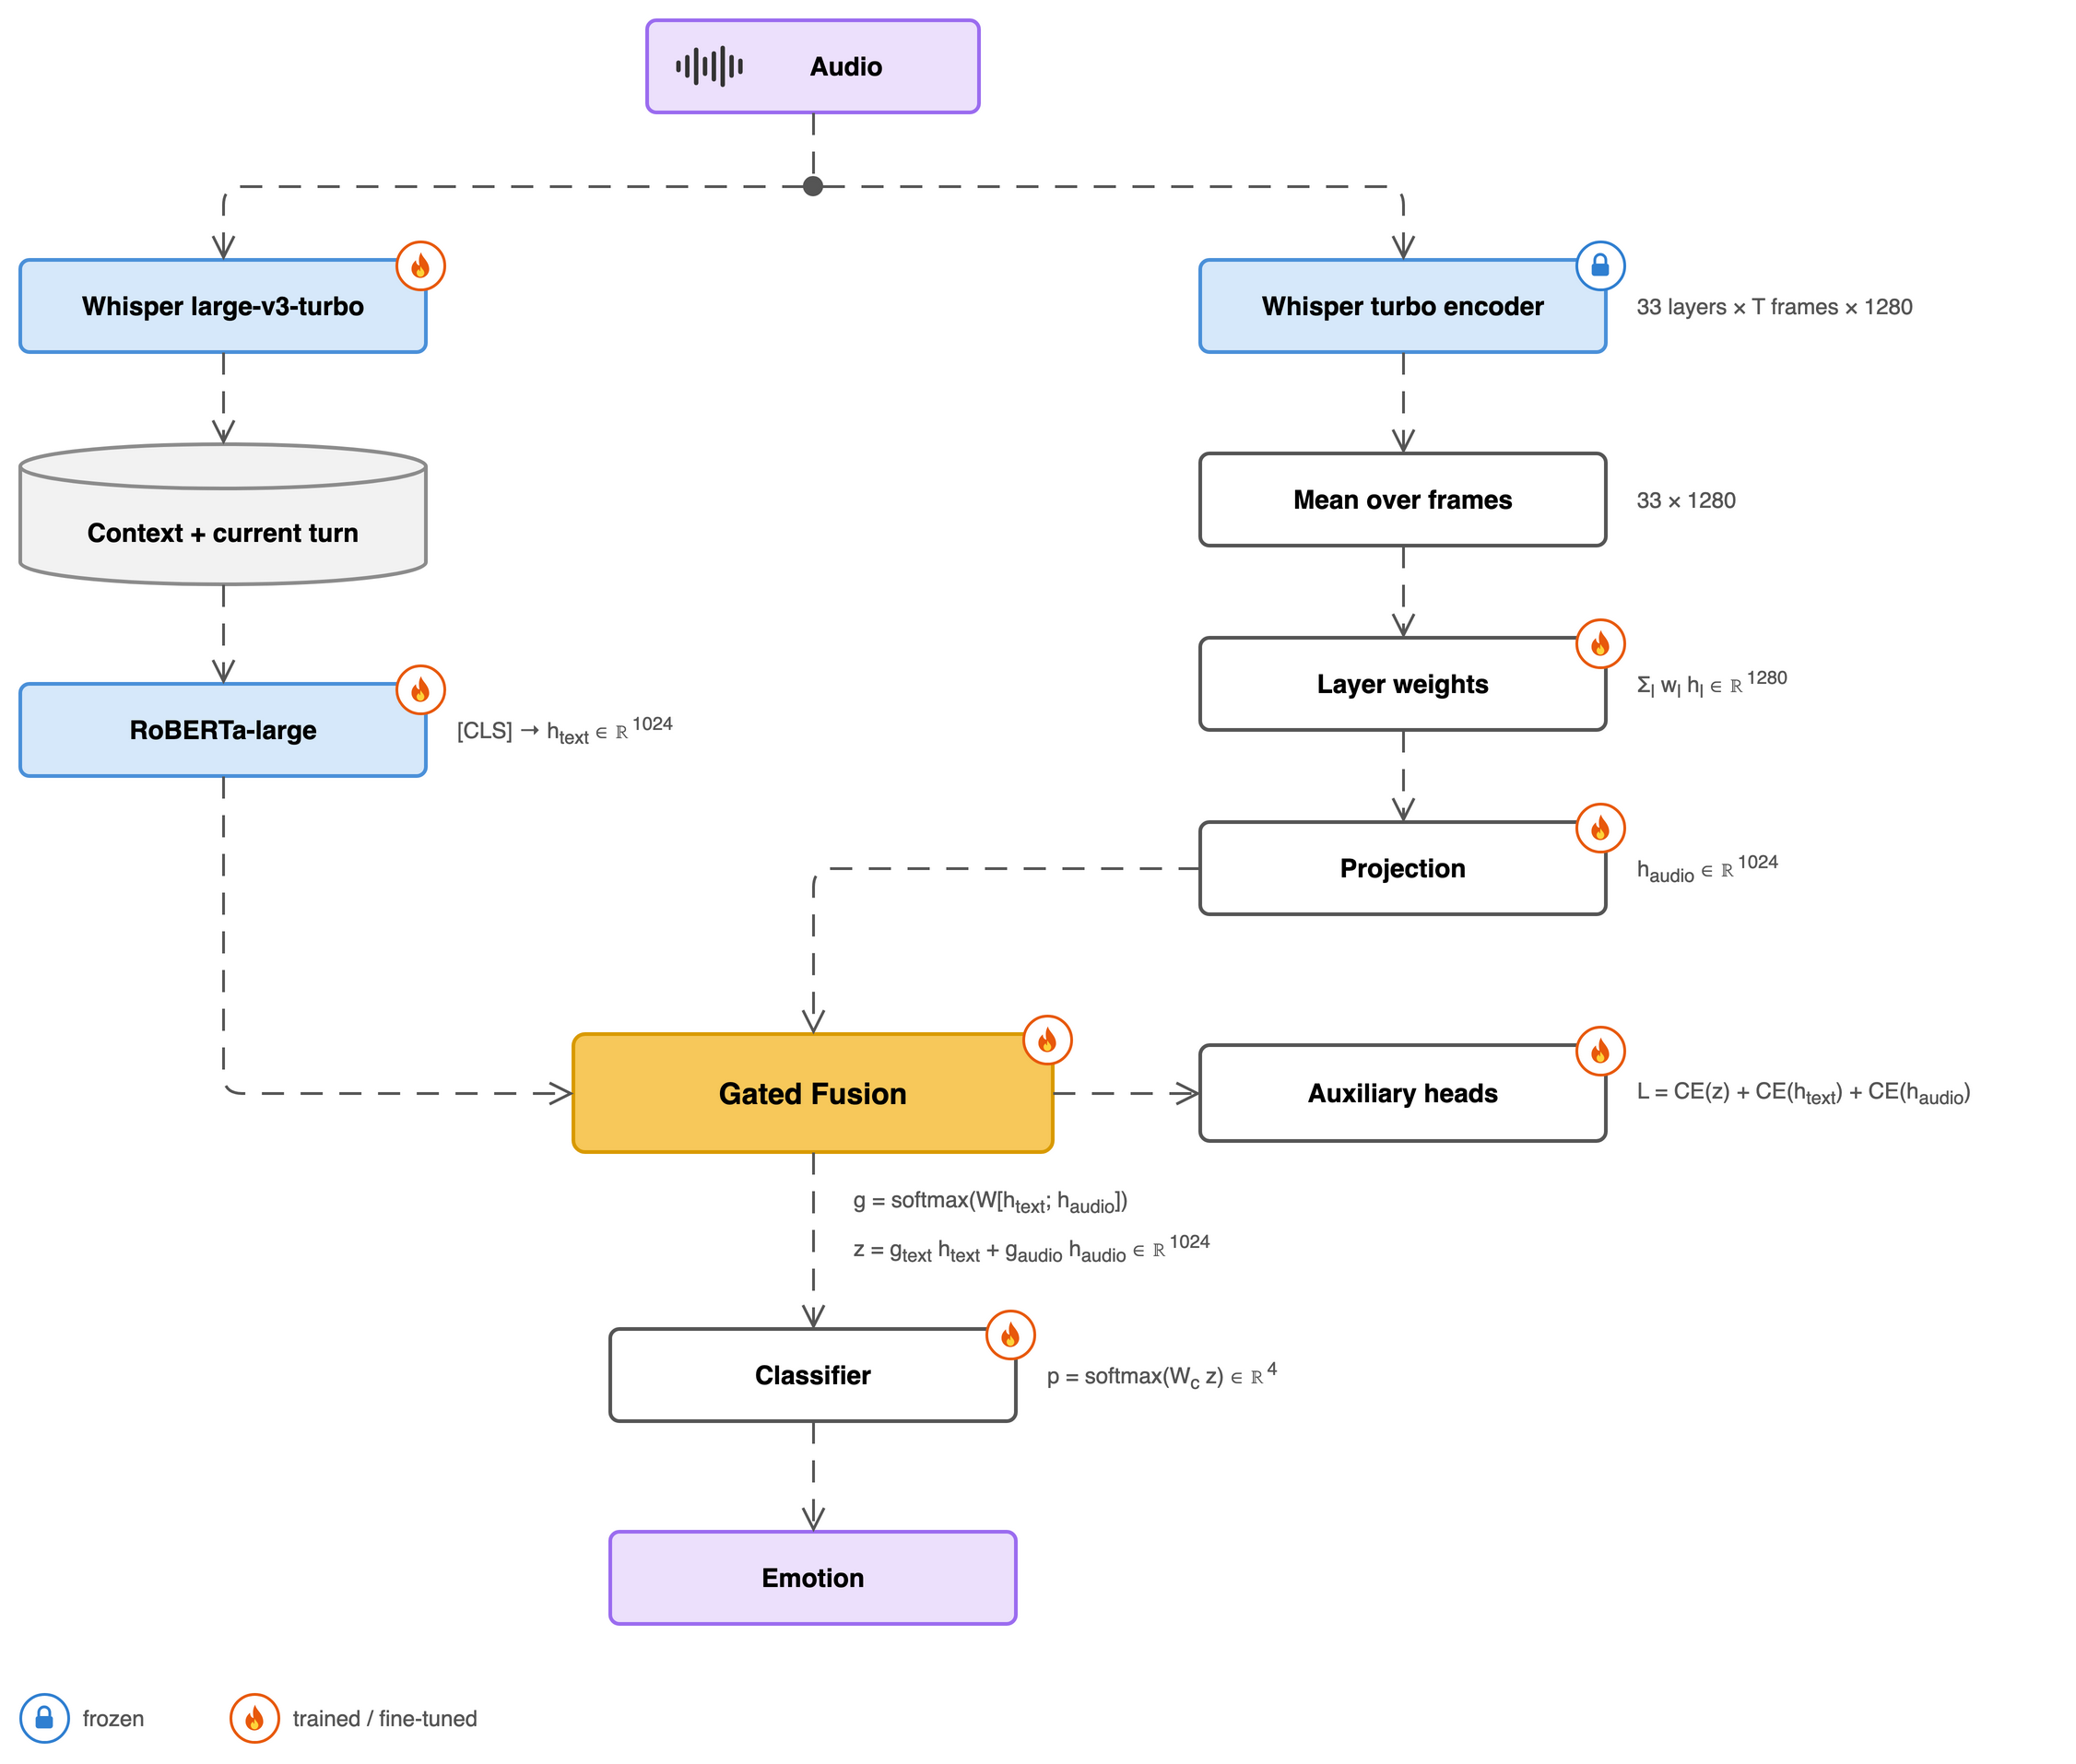
\includegraphics[width=0.58\textwidth]{figures/fig_flow.png}
\caption{One utterance through the model. $T$ is the number of encoder frames. A lock marks a frozen part and a flame
a trained part.}
\label{fig:flow}
\end{figure*}

\section{Data and Setup}

\textbf{Data.} IEMOCAP \cite{busso2008iemocap} has about 12 hours of dyadic conversations between ten actors in five
sessions, both scripted and improvised. We use the four standard classes, with excited merged into happy. This gives
5531 labeled turns out of 10039. The unlabeled turns are used only as context.

\begin{table}[!t]
\centering
\caption{Labeled turns per session and class.}
\label{tab:data}
\tabstyle
\begin{tabular}{lccccc}
\toprule
Session & Neutral & Happy & Angry & Sad & Total \\
\midrule
1 & 384 & 278 & 229 & 194 & 1085 \\
2 & 362 & 327 & 137 & 197 & 1023 \\
3 & 320 & 286 & 240 & 305 & 1151 \\
4 & 258 & 303 & 327 & 143 & 1031 \\
5 & 384 & 442 & 170 & 245 & 1241 \\
\midrule
Total & 1708 & 1636 & 1103 & 1084 & 5531 \\
\bottomrule
\end{tabular}
\end{table}

\textbf{Splitting.} We use leave-one-session-out cross-validation with five folds, so test speakers never appear in
training. In each fold, a random 10\% of the training sessions is the validation set that selects the best epoch.

\textbf{Metrics.} WER is computed with the Whisper English normalizer on both reference and hypothesis. For SER we
report unweighted accuracy (UA, the mean of per-class recall, our primary metric), weighted accuracy (WA) and weighted
F1. The best epoch is chosen on validation UA for SER and on validation WER for ASR. All results are means over the
five folds.

\textbf{Training.} We train on one NVIDIA L4 GPU. RoBERTa uses a learning rate of $10^{-5}$ and the new layers
$10^{-4}$, for 5 epochs with batch size 16. Each ASR model follows its standard finetuning recipe. SenseVoice-Small
trains for 10 epochs with a learning rate of $2\times10^{-4}$. Whisper large-v3-turbo is finetuned in full for 3
epochs with a learning rate of $10^{-5}$ and batch size 16. For Whisper, most of the validation WER gain comes in the
first epoch and the validation WER stops improving after the second, so three epochs are enough.

\section{Results}
\label{sec:results}

We build the system in four steps. Each step keeps the better option and passes it to the next.

\textbf{Steps 1--2: ASR model.} Table~\ref{tab:asr} compares SenseVoice-Small \cite{an2024funaudiollm} and Whisper
large-v3-turbo. Before finetuning, SenseVoice has the lower WER, with less than a third of the parameters. Whisper
gains much more from finetuning and ends lower, so the ASR model is finetuned Whisper large-v3-turbo. We use
SenseVoice-Small because the weights of SenseVoice-Large are not released. Table~\ref{tab:werEmo} breaks the
finetuned WER down by emotion. Happy turns are the hardest for both models and angry turns are the easiest. Whisper is lower on every class except happy. Its happy WER is raised by a failure on non-speech turns: on four test turns that contain only laughter or breathing (two of them happy, in sessions 1 and 3), the finetuned model repeats one token until the length limit. These four turns account for the higher WER of Whisper on sessions 1 and 3 (12.73\% and 14.37\%, against 4.72--8.27\% on the other sessions).

\begin{table}[!t]
\centering
\caption{Steps 1--2: WER (\%) before and after finetuning, on the test session, mean over 5 folds.}
\label{tab:asr}
\tabstyle
\begin{tabular}{lcccc}
\toprule
ASR model & Parameters & Original & Finetuned & Change \\
\midrule
SenseVoice-Small & 234M & \textbf{11.20} & 9.73 & $-1.47$ \\
Whisper large-v3-turbo & 809M & 13.19 & \textbf{9.56} & $-3.63$ \\
\bottomrule
\end{tabular}
\end{table}

\begin{table}[!t]
\centering
\caption{WER (\%) by emotion after finetuning.}
\label{tab:werEmo}
\tabstyle
\begin{tabular}{lcc}
\toprule
Emotion & SenseVoice-Small & Whisper large-v3-turbo \\
\midrule
Neutral & 10.5 & \textbf{8.4} \\
Happy & \textbf{12.5} & 16.0 \\
Angry & 6.8 & \textbf{4.7} \\
Sad & 8.4 & \textbf{7.8} \\
\bottomrule
\end{tabular}
\end{table}

\textbf{Step 3: audio encoder.} We fix the Whisper transcripts and the context, and compare two frozen encoders for
the audio branch (Table~\ref{tab:enc}). The Whisper encoder is higher on all three metrics, and the gate gives it
more weight. The average audio weight is 0.51 with the Whisper encoder and 0.28 with WavLM. This agrees with the EmoBox
benchmark \cite{ma2024emobox}. It also means that one Whisper checkpoint serves both the ASR model and the audio
branch.

\begin{table}[!t]
\centering
\caption{Step 3: frozen audio encoder in our system (\%). ``Whisper turbo'' is Whisper large-v3-turbo. ``Gate'' is the mean gate weight on the audio branch.}
\label{tab:enc}
\tabstyle
\begin{tabular}{lccccc}
\toprule
Audio encoder & UA & WA & W-F1 & $\Delta$UA & Gate \\
\midrule
WavLM-large \cite{chen2022wavlm} & 79.93 & 78.89 & 78.55 & $-1.24$ & 0.28 \\
Whisper turbo & \textbf{81.17} & \textbf{79.98} & \textbf{79.88} & -- & \textbf{0.51} \\
\bottomrule
\end{tabular}
\end{table}

\textbf{Step 4: ablation.} We remove one module at a time from the full system and train the rest in the same way
(Table~\ref{tab:abl}). Without audio, the model keeps only the text branch, RoBERTa-large with a classifier. Without context, the text input is the current turn alone and the audio branch is unchanged. Without text, the model keeps only the audio branch, which is the layer weights, the projection and the classifier.

\begin{table}[!t]
\centering
\caption{Step 4: ablation (\%). W-F1 is weighted F1. $\Delta$UA is the change in UA relative to our system.}
\label{tab:abl}
\tabstyle
\begin{tabular}{lcccc}
\toprule
System & UA & WA & W-F1 & $\Delta$UA \\
\midrule
Our system & \textbf{81.17} & \textbf{79.98} & \textbf{79.88} & -- \\
Without audio & 77.91 & 76.70 & 76.67 & $-3.26$ \\
Without context & 75.89 & 74.64 & 74.34 & $-5.28$ \\
Without text & 72.60 & 71.10 & 70.50 & $-8.57$ \\
\bottomrule
\end{tabular}
\end{table}

\section{Analysis}

\textbf{Which module matters most?} Removing text costs the most (8.57 UA), then context (5.28), then audio (3.26). Every module contributes: text the most, then context, then audio.

\textbf{How do ASR errors affect emotion recognition?} We keep the system fixed and change only the transcript
(Table~\ref{tab:gt}). Ground-truth text (0\% WER) gives 81.89 UA. Finetuned Whisper transcripts (9.56\% WER) give
81.17, which is 0.72 lower. Finetuned SenseVoice transcripts (9.73\% WER) give 81.29, which is 0.60 lower. Without
the audio branch the loss is similar. Ground-truth text gives 78.57 UA and Whisper transcripts give 77.91, a loss of
0.66. ASR errors at about 10\% WER therefore cost less than one UA point, with or without audio, while the audio branch
adds 3.26 UA and context adds 5.28. The two finetuned transcripts differ by 0.12 UA, in the opposite direction of their
WER gap of 0.17. Both differences are small next to the spread across folds, so UA does not separate the two ASR models
and we choose the ASR model on WER, which is its own task.

\begin{table}[!t]
\centering
\caption{Our system with three transcript sources (\%). $\Delta$UA is the change in UA relative to ground truth.}
\label{tab:gt}
\tabstyle
\begin{tabular}{lccc}
\toprule
Transcript & WER & UA & $\Delta$UA \\
\midrule
Ground truth & 0 & \textbf{81.89} & -- \\
Whisper, finetuned & 9.56 & 81.17 & $-0.72$ \\
SenseVoice, finetuned & 9.73 & 81.29 & $-0.60$ \\
\bottomrule
\end{tabular}
\end{table}

\textbf{What does each branch contribute?} In our system the gate puts on average 0.51 of the weight on audio, and
the value ranges from 0.44 to 0.63 across folds. Without context the text branch is weaker and the audio weight rises
to 0.71. With the WavLM encoder it falls to 0.28. Table~\ref{tab:recall} gives recall per class. Audio mainly helps
angry (+7.4). Context mainly helps happy (+9.8) and angry (+6.2). Sad recall changes least in every ablation.

\begin{table}[!t]
\centering
\caption{Recall per class (\%), mean over 5 folds.}
\label{tab:recall}
\tabstyle
\begin{tabular}{lcccc}
\toprule
System & Neutral & Happy & Angry & Sad \\
\midrule
Our system & \textbf{69.3} & \textbf{84.0} & \textbf{87.5} & \textbf{83.9} \\
Without audio & 66.6 & 81.6 & 80.1 & 83.4 \\
Without context & 65.8 & 74.2 & 81.3 & 82.2 \\
Without text & 62.1 & 67.1 & 80.7 & 80.4 \\
\bottomrule
\end{tabular}
\end{table}

\textbf{Is the gain consistent across folds?} Table~\ref{tab:folds} gives UA for each test session. Our system beats
``without audio'', ``without context'' and ``without text'' in all five folds. The Whisper encoder beats WavLM in
four of the five folds, all except session 5.

\begin{table}[!t]
\centering
\caption{UA (\%) per test session.}
\label{tab:folds}
\tabstyle
\begin{tabular}{lccccc}
\toprule
System & S1 & S2 & S3 & S4 & S5 \\
\midrule
Our system & \textbf{78.89} & \textbf{84.79} & \textbf{78.55} & \textbf{82.33} & 81.31 \\
WavLM encoder & 76.85 & 83.76 & 78.00 & 78.96 & \textbf{82.06} \\
Without audio & 75.02 & 82.88 & 75.99 & 75.64 & 80.00 \\
Without context & 75.81 & 73.47 & 70.81 & 79.63 & 79.71 \\
Without text & 70.05 & 75.49 & 71.06 & 70.76 & 75.63 \\
\bottomrule
\end{tabular}
\end{table}

\section{Conclusion}

We built an emotion-aware speech recognition system from two separate models and chose each part with a controlled
comparison. Finetuning reversed the ranking of the two ASR models, and Whisper large-v3-turbo reached 9.56\% WER. In
the emotion model, the encoder of the same Whisper checkpoint worked better than WavLM as the audio branch, so one
Whisper model serves both ASR and the audio branch. Text, context and audio each helped, text the most, and the
system reached 81.17\% UA. ASR errors at this rate cost 0.72 UA against ground-truth transcripts (0.66 UA without
audio), far less than the gain from the audio branch or from context. The finetuned Whisper still repeats tokens on
turns with only laughter or breathing, and detecting such turns before decoding is a simple next step. The system is evaluated on acted speech only. Spontaneous speech, for example MSP-Podcast, is left for future
work.

\bibliographystyle{IEEEtran}
\bibliography{refs}

\end{document}
